\documentclass{beamer}
\usepackage{../tut-slides}
\usepackage{../mathoperatorsAuD}

\usepackage{lmodern}
\usepackage{amsmath,amssymb}
\usepackage{wasysym}
\usepackage{stmaryrd}
\usepackage{enumerate}
%\usepackage[inline]{enumitem} 		%customize label
%\newcommand{\labelitemi}{\raisebox{1pt}{\scalebox{.9}{$\blacktriangleright$}}}
%\newcommand{\labelitemii}{$\vartriangleright$}
%\newcommand{\labelitemiii}{--}
\setbeamertemplate{itemize item}{\raisebox{1pt}{\scalebox{.9}{$\blacktriangleright$}}}
\setbeamertemplate{itemize subitem}{$\vartriangleright$}

\usepackage{booktabs}
\usepackage{tabularx}
\usepackage{tabu}
\newcommand*\head{\rowfont{\bfseries}}
\newcommand*{\tw}{\rowfont{\ttfamily}}
\renewcommand{\tabularxcolumn}[1]{>{\hspace{0pt}}m{#1}}
\usepackage{multirow}

\usepackage{cancel}

\usepackage{empheq}
\newcommand*\widefbox[1]{\fbox{\hspace{2em} #1 \hspace{2em}}}

\usepackage{tcolorbox}
\newtcolorbox{mymathbox}[1][]{colback=white, sharp corners, #1}

\usepackage{xcolor}
\usepackage{MnSymbol}

\newcommand{\col}[1]{\textcolor{cdpurple}{#1}}
\newcolumntype{R}[1]{>{\centering\arraybackslash}p{#1}}
\usepackage{tabularx}
\renewcommand{\tabularxcolumn}[1]{m{#1}}

\usepackage{ragged2e}
\usepackage{csquotes}

\DeclareMathOperator*{\argmax}{arg\,max}

%%%% EBNF-Terme %%%%
\usepackage{../syntaxdiagrammEBNF}


%%%% FARBEN %%%%%
\newcommand{\orange}[1]{\textcolor{cdorange}{#1}}
\newcommand{\green}[1]{\textcolor{cdgreen}{#1}}
\newcommand{\purple}[1]{\textcolor{cdpurple}{#1}}
\newcommand{\gray}[1]{\textcolor{cdgray}{#1}}

\begin{document}	
	\title{Algorithmen und Datenstrukturen}
	\subtitle{Übung 15: Wiederholung \& Konsultation}
	\author{Eric Kunze}
	\email{eric.kunze@tu-dresden.de}
	\city{TU Dresden}
%	\institute{Lehrstuhl für Grundlagen der Programmierung}
	\titlegraphic{
\includegraphics[width=2cm]{../TUD-white.pdf}}
	\date{31.01.2022}

	\maketitle

%%%%%%%%%%%%%%%%%%%%%%%%%%%%%%%%%%%%%%%%%%%%%%%%%%%%%%%%%%%%%%%%%%%%%%%%%%%%%%%%%%%

\section{Fixpunktsemantik}

\begin{frame} \frametitle{EBNF-Definition}
	
	\begin{center}
		\begin{tikzpicture}
		\node[baseline] (E) at (0,0) {$\mathcal{E}$}; 
		\node[baseline, right=1pt of E, inner sep=1pt] (eq) {$=$};
		\node[baseline, right=1pt of eq, inner sep=1pt] (ob) {$($}; 
		\node[right=2pt of ob, inner sep=1pt] (V) {$V,$}; 
		\node[right=2pt of V, inner sep=1pt] (Sigma) {$\Sigma,$}; 
		\node[right=2pt of Sigma, inner sep=1pt] (S) {$S,$}; 
		\node[right=2pt of S, inner sep=1pt] (R) {$R\phantom{,}\hspace{-3pt}$};
		\node[right=2pt of R, inner sep=1pt] {$)$};
		
		\node[align=right, below left=1mm and 1cm of V] (VText)
		{\scriptsize Nichtterminalsymbole};
		\path[->, bend right=15]  (VText.east) edge (V.south);
		
		\node[align=right, below left=7mm and 0mm of Sigma] (SigmaText)
		{\scriptsize Terminalsymbole};
		\path[->, bend right=15]  (SigmaText.north east) edge (Sigma.south);
		
		\node[align=left, below right=7mm and 0mm of S] (SText)
		{\scriptsize Startsymbol};
		\path[->, bend left=15]  (SText.north west) edge (S.south);
		
		\node[align=left, below right=1mm and 1cm of R] (RText)
		{\scriptsize Regelmenge};
		\path[->, bend left=15]  (RText.west) edge (R.south);
		
		
		\end{tikzpicture}
	\end{center}
	
	\small
	
	Jede \textbf{EBNF-Regel} besteht aus einer linken und einer rechten Seite, die rechte Seite ist ein \textbf{EBNF-Term}.
	\begin{equation*}
	\text{\textit{Nichtterminalsymbol}} ::= \text{\textit{EBNF-Term}}
	\end{equation*}
	
	\pause
	
	\textbf{Definition (EBNF-Terme)}:	
	Seien $V$ (syntaktische Variablen) und $\Sigma$ (Terminalsymbole) endliche Mengen mit $V \cap \Sigma = \emptyset$. Die Menge der EBNF-Terme über $V$ und $\Sigma$ (notiere: $T(\Sigma, V)$), ist die \emph{kleinste} Menge $T \subseteq \brackets{V \cup \Sigma \cup \menge{\hat{\{}, \hat{\}}, \hat{[}, \hat{]}, \hat{(}, \hat{)}, \hat{|}}}$ mit $V \subseteq T$, $\Sigma \subseteq T$ und
	\begin{itemize}
		\item Wenn $\alpha \in T$, so auch $\rdb{\alpha} \in T$, $\wdh{\alpha} \in T$, $\byp{\alpha} \in T$.
		\item Wenn $\alpha_1, \alpha_2 \in T$, so auch $\opt{\alpha_1}{\alpha_2} \in T$, $\alpha_1 \alpha_2 \in T$.
	\end{itemize}
\end{frame}

\begin{frame} \frametitle{Übersetzung EBNF $\leftrightarrow$ Syntaxdiagramme}
	\small
	Sei $v \in V$ und $w \in \Sigma$. $trans(v) =$ 
	\scalebox{0.7}{
		\tikz[baseline=-0.5ex]{\coordinate (start) at (0,0); \coordinate (end) at (2,0); \nonterminal{v}{$v$}{(1,0)}; \draw[thick] (start) -- (v) -- (end);}
	};
	$trans(w) =$ 
	\scalebox{0.7}{
		\tikz[baseline=-0.5ex]{\coordinate (start) at (0,0); \coordinate (end) at (2,0); \terminal{w}{$w$}{(1,0)}; \draw[thick] (start) -- (w) -- (end);}
	}
	
	Sei $\alpha \in T(\Sigma, V)$ ein EBNF-Term. 
	\begin{itemize}
		\item \makebox[2cm][l]{$trans(\ \wdh{\alpha} \ )$} $=$  
		\scalebox{0.7}{
			\tikz[baseline=-0.5ex]{
				\coordinate (start) at (0,0); 
				\coordinate (end) at (4,0);
				\coordinate (mid) at (2,0); \terminals{alpha}{$trans(\alpha)$}{(2,-1)}; 
				\draw[thick] (start) 
				-- coordinate[pos=0.3](l-start) (mid)
				-- coordinate[pos=0.7](l-end) (end);
				\loopleft{alpha}{l-start} 
				\loopright{l-end}{alpha}
			}
		}
		%
		\item \makebox[2cm][l]{$trans(\ \byp{\alpha} \ )$} $=$  
		\scalebox{0.7}{
			\tikz[baseline=-0.5ex]{
				\coordinate (start) at (0,0); 
				\coordinate (end) at (4,0);
				\coordinate (lower) at (2,-1); \terminals{alpha}{$trans(\alpha)$}{(2,0)}; 
				\draw[thick] (start) 
				-- coordinate[midway](l-start) (alpha)
				-- coordinate[midway](l-end) (end);
				\altleft{l-start}{lower}
				\altright{lower}{l-end}
			}
		}
		%
		\item $trans(\ \rdb{\alpha} \ ) = trans(\alpha)$
	\end{itemize}
	
	Seien $\alpha_1, \alpha_2 \in T(\Sigma, V)$ zwei EBNF-Terme. 
	\begin{itemize}
		\item $trans(\ \alpha_1 \alpha_2 \ ) =$  
		\scalebox{0.7}{
			\tikz[baseline=-0.5ex]{
				\coordinate (start) at (0,0); 
				\coordinate (end) at (6,0); \terminals{alpha1}{$trans(\alpha_1)$}{(2,0)}; 
				\terminals{alpha2}{$trans(\alpha_2)$}{(4,0)}; 
				\draw[thick] (start) 
				-- (alpha1)
				-- (alpha2)
				-- (end);
			}
		}
		
		\item $trans(\ \opt{\alpha_1}{\alpha_2} \ ) =$  
		\scalebox{0.7}{
			\tikz[baseline=-0.5ex]{
				\coordinate (start) at (0,0); 
				\coordinate (end) at (4,0); \terminals{alpha1}{$trans(\alpha_1)$}{(2,0)}; 
				\terminals{alpha2}{$trans(\alpha_2)$}{(2,-1)}; 
				\draw[thick] (start) 
				-- coordinate[midway](l-start) (alpha1)
				-- coordinate[midway](l-end) (end);
				\altleft{l-start}{alpha2}
				\altright{alpha2}{l-end}
			}
		}
	\end{itemize}
	
	\tiny Auszug aus dem Foliensatz der Vorlesung
\end{frame}

\begin{frame} \frametitle{Semantik von EBNF-Termen}
	\small
	\textbf{Ziel:} Ordne einer EBNF-Definition $\mathcal{E} = (V,\Sigma,S,R)$ ihre Sprache zu
	\begin{itemize}
		\item $W(\mathcal{E}, v)$ bezeichnet von $v \in V$ beschriebene Objektsprache
		\item $\rho \colon V \to \pows{\Sigma^\ast}$ ordnet jeder syntaktischen Variable $v \in V$ eine Sprache zu 
		\item Vorstellung: $\rho(v)$ ist bestes Wissen über die von $v$ beschriebene Sprache
	\end{itemize}
	\pause
	
	\textbf{Problem:} Wie bekomme ich aus einem EBNF-Term eine Sprache? 
		
	Semantik $\abb{\sem{\cdot}}{\underbrace{T(\Sigma, V)}_{\text{EBNF-Term } \alpha}}{((\underbrace{V \to \pows{\Sigma^\ast}}_{\rho}) \to \pows{\Sigma^\ast})}$
\end{frame}

\begin{frame} \frametitle{Semantik von EBNF-Termen}
	\begin{equation*}
		\abb{\sem{\cdot}}{\underbrace{T(\Sigma, V)}_{\text{EBNF-Term } \alpha}}{((\underbrace{V \to \pows{\Sigma^\ast}}_{\rho}) \to \pows{\Sigma^\ast})}
	\end{equation*}
	
	Sei $\alpha \in T(\Sigma, V)$ ein EBNF-Term. Die Semantik  $\sem{\alpha}(\rho)$ von $\alpha$ ist definiert als:
	\begin{itemize}
		\item Wenn $\alpha = v \in V$, dann gilt $\sem{\alpha}(\rho) = \rho(v)$.
		\item Wenn $\alpha = w \in \Sigma$, dann gilt $\sem{\alpha}(\rho) = \menge{w}$.
		\medskip
		\item Wenn $\alpha = \wdh{\alpha_1}$, dann gilt $\sem{\alpha}(\rho) = \brackets{\sem{\alpha_1}(\rho)}^\ast$.
		\item Wenn $\alpha = \byp{\alpha_1}$, dann gilt $\sem{\alpha}(\rho) = \sem{\alpha_1}(\rho) \cup \menge{\epsilon}$.
		\item Wenn $\alpha = \rdb{\alpha_1}$, dann gilt $\sem{\alpha}(\rho) = \sem{\alpha_1}(\rho)$.
		\medskip
		\item Wenn $\alpha = \alpha_1 \alpha_2$, dann gilt $\sem{\alpha}(\rho) = \sem{\alpha_1}(\rho) \cdot \sem{\alpha_2}(\rho)$.
		\item Wenn $\alpha = \opt{\alpha_1}{\alpha_2}$, dann gilt $\sem{\alpha}(\rho) = \sem{\alpha_1}(\rho) \cup \sem{\alpha_2}(\rho)$.
	\end{itemize}
\end{frame}

\begin{frame} \frametitle{Fixpunktiteration -- eine Analogie}
	\small
	\textbf{Ausblick:} Fixpunktiteration zur Nullstellenbestimmung
	
	Gegeben sei eine Funktion $g \colon \R \to \R$, von der wir eine Nullstelle suchen, d.h. ein $\quer{x} \in \R$ mit $g(\quer{x}) = 0$.
	
	\pause
	\textbf{Methode:} Newtonverfahren --- definiere $\Phi(x) \defeq x - \frac{g(x)}{g'(x)}$.
	\begin{itemize}
		\item Starte mit \enquote{beliebigem} Startwert $x_0 \in \R$.
		\item Berechne stets $x_{i+1} = \Phi(x_i)$.
	\end{itemize}

	\pause
	
	\begin{minipage}{\dimexpr0.6\linewidth-\fboxrule-\fboxsep}
		\textbf{Beobachtung:} \\
		$x_{i}$ nähert sich der Nullstelle $\quer{x}$ an
		
		\pause \smallskip
		Ein \textit{Fixpunkt} von $\Phi$ ist ein Punkt $x$ mit $\Phi(x) = x$.
		
		\pause \smallskip
		Die Nullstelle $\quer{x}$ ist ein Fixpunkt von $\Phi$, da
		\begin{equation*}
		\Phi(\quer{x}) = \quer{x} - \frac{g(\quer{x})}{g'(\quer{x})} = \quer{x} .
		\end{equation*} 
	\end{minipage}
	\pause
	\begin{minipage}{\dimexpr0.4\linewidth-\fboxrule-\fboxsep}
		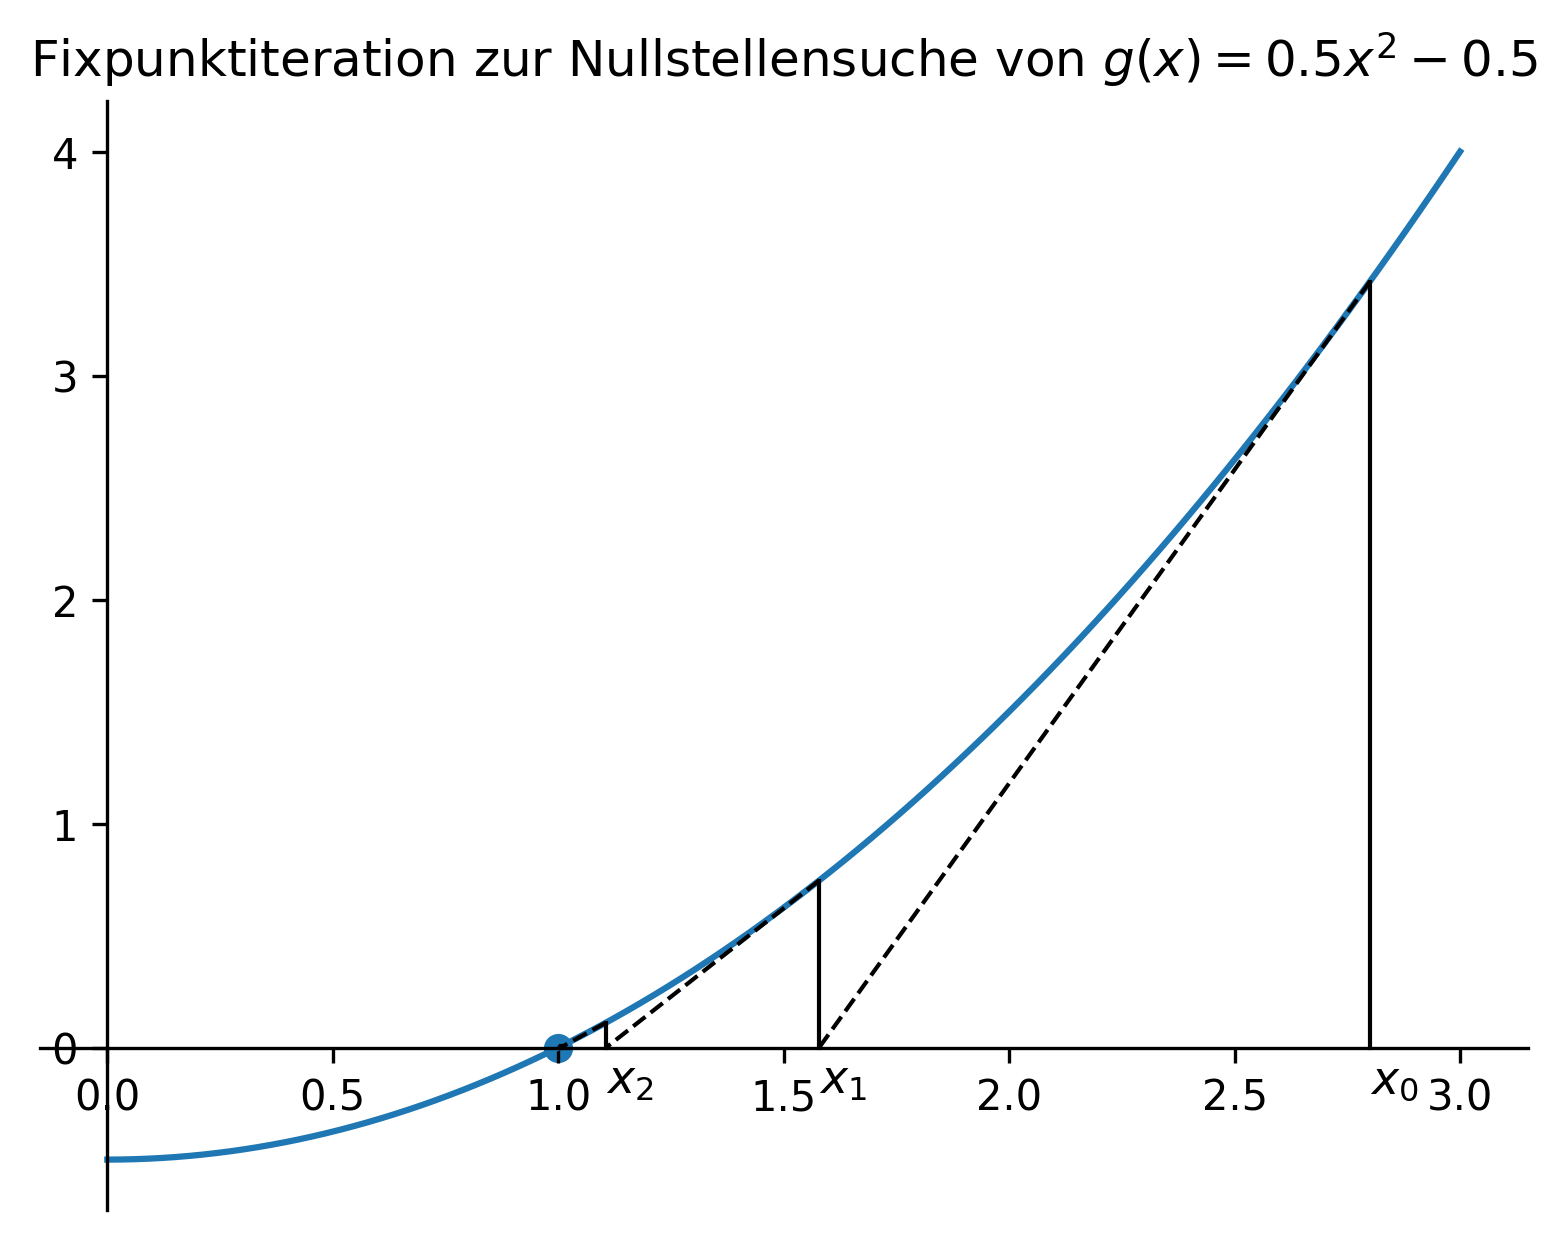
\includegraphics[width=\linewidth]{../tut03/tut03_fixpunktiteration.png}
	\end{minipage}
	
\end{frame}

\begin{frame} \frametitle{Fixpunktiteration für EBNF}
	\small
	\textbf{Ziel:} berechne Sprache $W(\mathcal{E}, v)$ für alle $v \in V$ einer EBNF-Definition $\mathcal{E} = (V, \Sigma, S, R)$.
	
	\pause
	Iterierende Funktion:
	\begin{equation*}
		f \colon \underbrace{\brackets{V \to \pows{\Sigma^\ast}}}_{\rho} \to \brackets{V \to \pows{\Sigma^\ast}}
	\end{equation*}
	
	\begin{itemize}
		\item Starte mit bisherigen Kenntnis $\rho(v) = \emptyset$ für alle $v \in V$. \\
		(Nichtswissen)
		\item Berechne stets neues Wissen $\rho_{\text{neu}} = f(\rho_{\text{alt}})$. \\
		(Generiere neues Wissen)
	\end{itemize}

	\pause
	\textbf{Ende:} erreiche einen Fixpunkt $\rho$ mit $f(\rho) = \rho$
	
	Dann gilt $\rho(v) = W(\mathcal{E}, v)$ für alle $v \in V$.
\end{frame}

\begin{frame} \frametitle{Fixpunktiteration für EBNF}
	Da $V$ endlich ist, ist $f(\rho) \colon V \to \pows{\Sigma^\ast}$ nur auf endlich vielen Argumenten definiert, deren Bilder wir nun als Spaltenvektor schreiben:
	\begin{equation*}
		\left(
		\begin{array}{c}
			f(\rho)(v_1) \\
			f(\rho)(v_2) \\
			\vdots \\
			f(\rho)(v_n)
		\end{array}
		\right)
		\begin{array}{c}
			\in \pows{\Sigma^\ast} \\
			\in \pows{\Sigma^\ast} \\
			\vdots \\
			\in \pows{\Sigma^\ast}
		\end{array}
	\end{equation*}
	
	\pause
	Ein Iterationsprozess lässt sich dann wie folgt notieren:
	\begin{align*}
		\begin{pmatrix} \emptyset \\ \emptyset \end{pmatrix}
		\overset{f}{\mapsto^1}
		\begin{pmatrix} f(\rho)(v_1) \\ f(\rho)(v_2) \end{pmatrix}
		&\overset{f}{\mapsto^2}
		\begin{pmatrix} f(f(\rho))(v_1) \\ f(f(\rho))(v_2) \end{pmatrix}
		\overset{f}{\mapsto^3}
		\dots \\
		&\overset{f}{\mapsto^n}
		\begin{pmatrix} f^n(\rho)(v_1) \\ f^n(\rho)(v_2) \end{pmatrix}
		\overset{f}{\mapsto^{n+1}}
		\dots
	\end{align*}
\end{frame}


\section{Pulsierender Speicher}

\begin{frame} \frametitle{Pulsierender Speicher}
	\small
	\textbf{Gültigkeitsbereiche von Objekten}:
	\begin{itemize}
		\item Eine Funktion ist ab ihrer Deklaration bis zum Programmende sichtbar. Vorwärtsdeklarationen beachten!
		\item  Ihre formalen Parameter jedoch nur innerhalb der Funktionsdefinition!
		\item Gibt es gleichlautende formale Parameter in verschiedenen Funktionen, müssen diese in der Tabelle natürlich unterschieden werden (z.B. durch \enquote{x in f}).
		\item Vorsicht bei Namenskonflikten: lokale Variablen überschreiben die Sichtbarkeit globaler Variablen.
	\end{itemize}
\end{frame}

\begin{frame} \frametitle{Pulsierender Speicher}
	\small
	\textbf{Speicherprotokoll}:
	\begin{itemize}
		\item Für jeden Funktionsaufruf werden erst die Parameter, dann die lokalen Variablen in Reihenfolge ihres Auftretens in der Umgebung notiert. Globale Variablen stehen ganz vorn.
		\item Variablennamen werden nur notiert, wenn die Variablen sichtbar sind. Globale Variablennamen werden immer notiert.
		\item Der Wert von nicht sichtbaren Variablen muss nur notiert werden wenn er sich ändert.
		\item Uninitialisierte Variablen werden mit Inhalt \enquote{?} notiert.
	\end{itemize}
\end{frame}

\section{Prozessproblem}

\begin{frame} \frametitle{Floyd-Warshall $\to$ Aho-Hopcraft-Ullmann}
	\small
	modifizierte Adjazenzmatrix
	\begin{equation*}
		mA_G = \begin{cases}
			A_G(u,v) & \text{wenn } u \neq v \\
			A_G(u,v) \oplus \mathbf{1} & \text{wenn } u = v
		\end{cases}
	\end{equation*}

	\textbf{Initialisierung}: $D_G^{(0)} = mA_G$

	\textbf{Rekursion}:
	\begin{equation*} \small
	\boxed{\begin{aligned}
		&D_G^{(k+1)}(u,v) \\
		= \enskip &D_G^{(k)}(u,v) \textcolor{cdorange}{\oplus} \brackets{D_G^{(k)}(u,k+1) \textcolor{cdpurple}{\odot} (D_G^{(k)}(k+1,k+1))^\ast \textcolor{cdpurple}{\odot} D_G^{(k)}(k+1,v)}
		\end{aligned}}
	\end{equation*}
	
	\textcolor{cdgray!70}{%
		vgl. dazu Floyd-Warshall:
		\begin{equation*}
			\begin{aligned}
				&D_G^{(k+1)}(u,v) \\
				= \enskip &\textcolor{cdorange}{\min}\menge{D_G^{(k)}(u,v) , D_G^{(k)}(u,k+1) \,
				\textcolor{cdpurple}{\boldsymbol{+}} \,
				0 \,
				\textcolor{cdpurple}{\boldsymbol{+}} \,
				D_G^{(k)}(k+1,v)}
			\end{aligned}
		\end{equation*}}
\end{frame}

\end{document}
